\documentclass[12pt]{article}
\usepackage{geometry}             
\usepackage{moreverb}   
\usepackage{fancyhdr}
\geometry{letterpaper}
\usepackage{algorithmic}             
\usepackage{algorithm}
\usepackage{array}     
\usepackage{hyperref}
\usepackage{graphicx}
\usepackage{subfigure}
\usepackage{fullpage}
\usepackage{amsmath, amssymb, amsthm}
\usepackage[framed,numbered,autolinebreaks,useliterate]{mcode}
\usepackage{mathabx}
\usepackage{float}

\newtheorem{theorem}{Theorem}
\newtheorem{corollary}{Corollary}
\newtheorem{proposition}{Proposition}
\newtheorem{lemma}{Lemma}
\newtheorem{definition}{Definition}
\newtheorem{remark}{Remark}
\newtheorem{notation}{Notation}

% my macros
\newcommand{\paren}[1]{\left({#1}\right)}
\newcommand{\bracket}[1]{\left[{#1}\right]}
\newcommand{\curly}[1]{\left\{{#1}\right\}}
\newcommand{\vecb}[1]{\mathbf{#1}}
\newcommand{\matb}[1]{\mathbf{#1}}
\newcommand{\V}[1]{\mathbf{#1}}
\newcommand{\m}[1]{\mathbf{#1}}
\newcommand{\inhomog}[1]{\widetilde{#1}}
\newcommand{\transpose}[1]{{#1}^\top}

\begin{document}

\title{CS 283 Final Project \\ Pipeline for Improving Accuracy of Hand Tracking}
\date{Fall 2012}
\author{Kenny Yu, HUID: 30798260}

\maketitle

%%%%%%%%%%%%%%%%%%%%%%%%%%%%%%%%%%%%%%%%%%%%%%%%%%%%%
\section{Introduction}
What if you had the power of Microsoft's Kinect in your webcam? What if you could control applications simply with a swipe of your hand? Detecting and tracking hands typically requires a good detector, which requires large amounts of good data (typically at least 5000 images !!!CITE!!!) and a tremendous amount of computation time to train the classifier. In this paper, we trained our hand detector with only 250 images, generated from 10 positives and 100 negatives. Despite this poorly trained Haar cascade classifier, we provide a pipeline to improve accuracy during hand tracking, providing comparable results to tracking with a  well-trained hand detector.

\section{Methods}

\subsection{Generating our Hand Detector}

\noindent\begin{figure}[H]
\centering
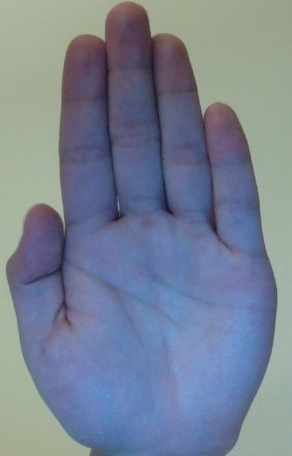
\includegraphics[width=50px, height=90px]{../data/positives/img0000.jpg}
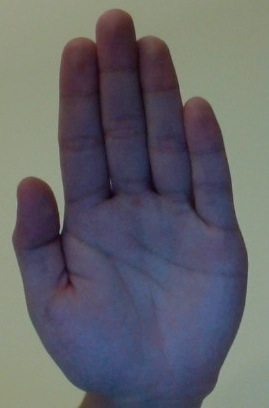
\includegraphics[width=50px, height=90px]{../data/positives/img0001.jpg}
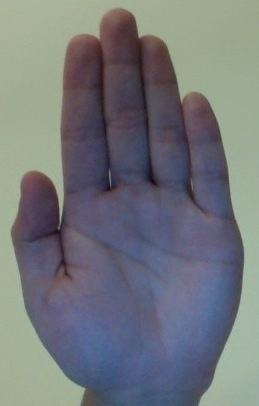
\includegraphics[width=50px, height=90px]{../data/positives/img0002.jpg}
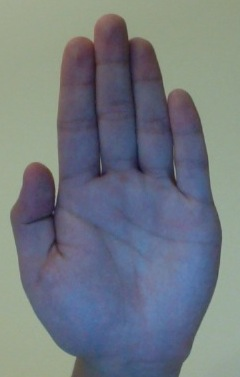
\includegraphics[width=50px, height=90px]{../data/positives/img0003.jpg}
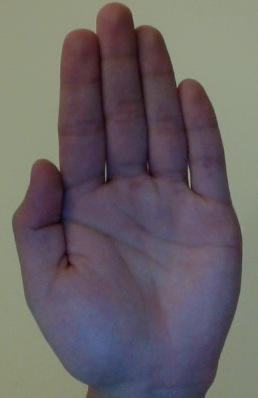
\includegraphics[width=50px, height=90px]{../data/positives/img0004.jpg} \\
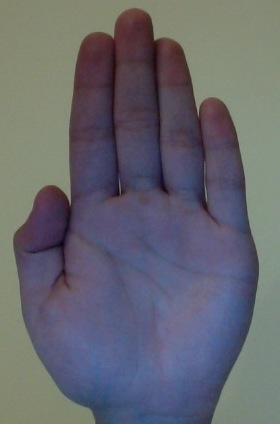
\includegraphics[width=50px, height=90px]{../data/positives/img0005.jpg}
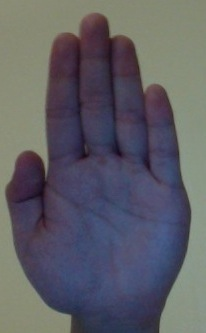
\includegraphics[width=50px, height=90px]{../data/positives/img0006.jpg}
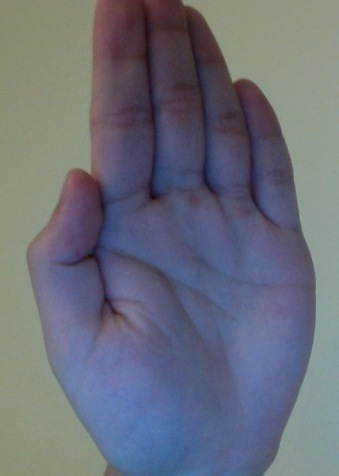
\includegraphics[width=50px, height=90px]{../data/positives/img0007.jpg}
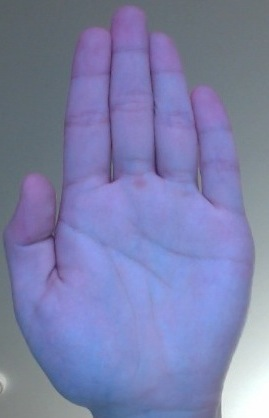
\includegraphics[width=50px, height=90px]{../data/positives/img0008.jpg}
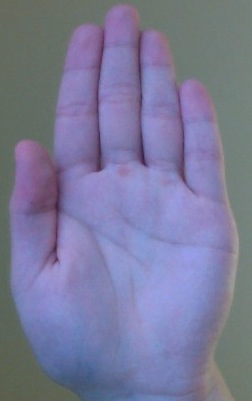
\includegraphics[width=50px, height=90px]{../data/positives/img0009.jpg}
\caption{The 10 positive images used to train our hand detector. We generated 250 samples from these, each of size 90 pixels high and 50 pixels wide.}
\label{traininghands}
\end{figure}

To generate our hand detector, we took 10 pictures of our right hand using a webcam from a  Macbook Pro 2011 model, and we cropped the images to leave only our hand in the images. Our pictures consisted of our right hand with the palm facing forward and all fingers together. See Figure \ref{traininghands} for the the images we used as positives. We used the first 100 images from !!!!CITE!!!!! as negatives. We used OpenCV's \texttt{opencv\_createsamples} !!! CITE !!!!! utility to generate 250 90 $\times$ 50 pixel samples from this set of 10 positives and 100 negatives, resulting in images where our positive images have been warped by homographies and placed randomly into our negative images. We used OpenCV's \texttt{opencv\_haartraining} tool to train our Haar cascade classifier, setting our min hit rate to $0.999$, our max false alarm rate to $0.5$ and with 14 stages in our cascade. This took about a day to complete.

\subsection{Building the Pipeline}

\section{Results}

\section{Conclusions}

\section{References}

\end{document}